\section{Methods} \label{section:methods}

\subsection{Proposed Pipeline}
To address the posed research questions, the following pipeline is proposed. Note that these stages might be modified later on as the project progresses and new needs are identified. The objective of reducing memory usage and training time remain the same regardless of the change.\\
These are shown in Figure \ref{fig:process}. This figure is purely for demo and the images shown do not reflect the ones that will be used in the project. The thresholded image was created using Photoshop and is not an output of any kind so far.

\begin{figure}[htbp]
    \centering
    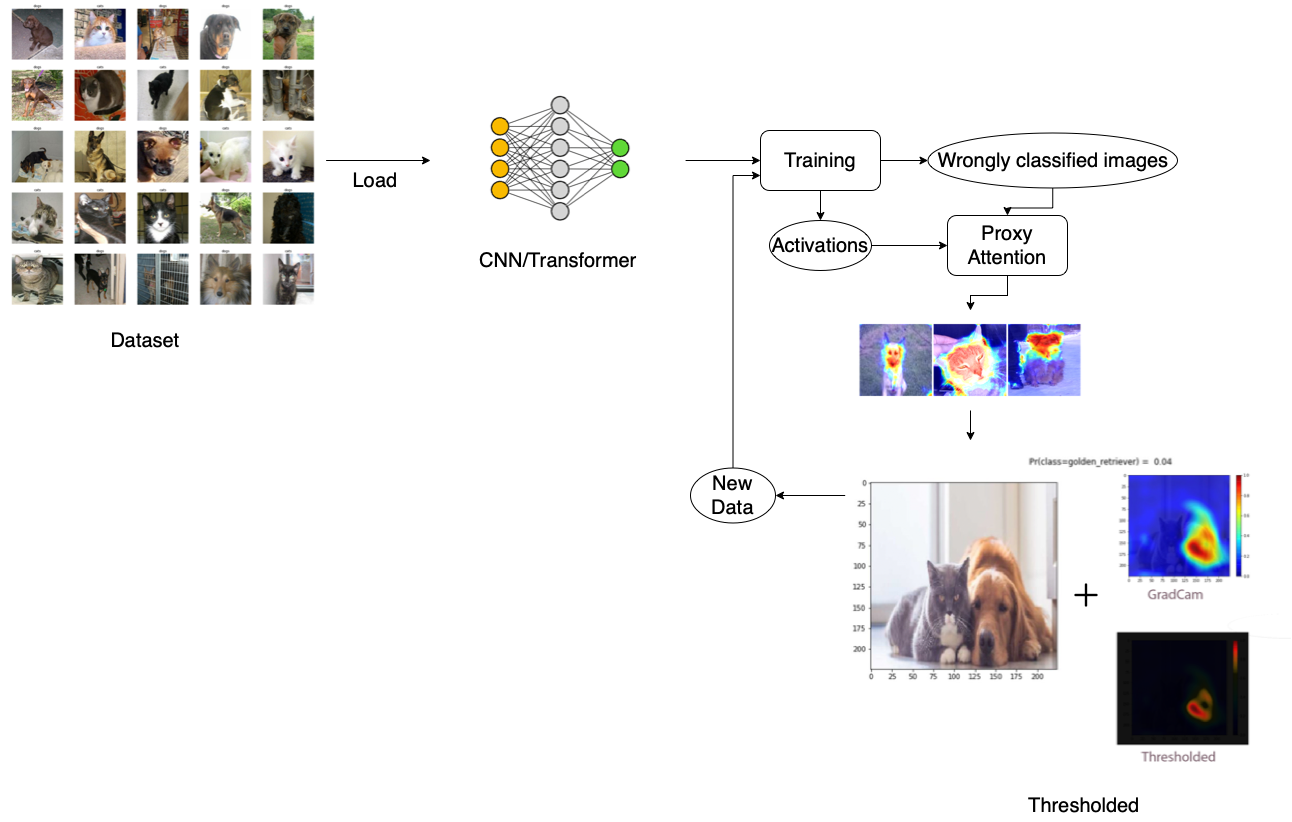
\includegraphics[width=.9\textwidth]{images/thesis_report.drawio.png}
    \caption{Visualizing the Process}
    \label{fig:process}
\end{figure}

\subsubsection*{Stage 0 - Setup}
Since there are a lot of experiments to be run, a configuration file is created with all the parameters required per network and data. Every dataset has it's own path, definition of labels, and image sizes. To ensure compatibility with future research, this type of configuration is very important. Specific Dataloaders for each configuration will have to be created.
To ensure proper comparision, the images will all be resized to a common size of 224x224. 

\subsubsection*{Stage 1 - Intial Training}
The first stage of the main pipeline is pre-training. This will be done by fine tuning the model on the chosen dataset by transfer learning from a pretrained ImageNet model, if it exists for the chosen model. The number of epochs to train here is yet to be decided. Once this initial training is done, the model is saved for the next stage and the memory is cleared to prevent the GPU from being overloaded.
While training, the gradients for the final layer could be saved using Pytorch Hooks which is just a means to "hook" into the training pipeline and insert arbitrary computation steps.

\subsubsection*{Stage 2 - Proxy Attention}
The Proxy Attention stage involves first identifying the images that the model incorrectly classified from the training data. Note that this is not an inference step, but an intermediate, therefore validation data is not used now. After these images are identified, the activations of the final layer wrt each of these images is computed and reshaped into a "map" with the same size of the image. The highest values of this activation map are thresholded, and these locations are mapped back onto the original image. In the original image, these areas of high activations are replaced with a black pixel. These images are then saved to the disk.

\subsubsection*{Stage 3 - Retraining}
Stage 1 is repeated with the new data along with the original images. Until a satsifactory performance is achieved, this loops back to Stage 1.

\subsection{Frameworks}
The existing frameworks that will be used to speed up this research effort are as follows: 
\begin{itemize}
\item Pytorch \cite{paszke2019pytorch}: For the entire deep learning backbone
\item OpenCV \cite{bradski2000opencv}: For optimized reading of images
\item Fastai \cite{howard2018fastai}: A wrapper on Pytorch that enables faster experimentation 
\end{itemize}

\subsection{Dataset and Models}
The Datasets and Models to be used are yet to be decided. But in general, the evaluation will start with simpler datasets like the \href{https://www.kaggle.com/datasets/grassknoted/asl-alphabet}{American Sign Language dataset} and move onto more complex ones.
The same applies to the models. Intial experiments will start with ResNet \cite{he2016deep} and move on to more complex models. Eventually the ViT \cite{dosovitskiy2020image} will also be used.

\subsection{Evaluation}
Evaluation is one of the most important steps to the pipeline in this project. The following metrics are considered now, but research needs to be done on which to include and other metrics to be added. \\
It is intended that we test around 3 XAI algorithms and 3 datasets. (These have not been researched just yet but will be in the starting weeks of the project)
\begin{itemize}
    \item The Accuracy, Precision and Recall of the predictions on the validation set
    \item The time taken to train as compared to the same network without Proxy Attention
    \item Comparision with ViT \cite{dosovitskiy2020image} and the presence/abscence of Attention
    \item The amount of GPU RAM used for training
\end{itemize}
These metrics have to be added into the pipeline to avoid having to manually compute them.

\subsection{Tackling Potential Issues}
Since this is still an experimental procedure, some issues come to mind. This section aims to provide some answers to them. It is to be noted that further issues may rise during implementation, but these are not known as of now and will be brought to light in time.
\subsubsection*{Memory Constraints}
To reduce memory usage we use the following measures.
\begin{enumerate}
    \item Unloading the model and it's weights after every stage so it stops using the GPU RAM.
    \item Saving the augmented images to the disk instead of keeping them in memory.
    \item Using Mixed Precision Training whereby most of the computation is performed in 16bit floats instead of the usual 32bits.
    \item Using transfer learning throughout the process.
\end{enumerate}
\subsubsection*{Computation Time for Activations}
Computing the activations can be costly, so some measures will be taken to overcome them.
\begin{enumerate}
    \item Attempt to parallelize the final prediction over all the images in a batch.
    \item Use Pytorch hooks to pre compute these activations as in part they would be computed during training.
\end{enumerate}
\subsubsection*{Accuracy vs Confidence}
While attempting to flesh out this idea, we realized that that it would be interesting to utilize the confidence of predictions along with the accuracy in order to see if this made any difference. This will possibly be discussed in the future.